\section{Implementierung von Event-Sourcing}
\label{sec:implementation:eventSouring}
Die Persistierung der Daten basiert auf dem \textit{Event-Sourcing}, wie in Abschnitt \ref{sec:eventSourcing} beschrieben wird. Das Prinzip von \textit{Event-Sourcing} ist es, aufgetretene Ereignisse abzuspeichern und gegebenenfalls wieder einzuspielen, um so einen Zustand reproduzieren und nachvollziehen zu können \citep{betts2013CQRSEventSourcing}. \\
Das verwendete Framework \textit{Akka.NET} bietet eine grundlegende Unterstützung für \textit{Event-Sourcing} \citep{Akka.NETCommunityAkka.NETDocumentation}. Dabei werden Events als Nachrichten repräsentiert, welche dem Framework übergeben und anschließend abgespeichert werden. 
Erst nach erfolgreicher Speicherung des Events, kann auf das Event selber reagiert werden. Dadurch wird verhindert, dass Aktionen zu Events ausgeführt werden, jedoch das Event nicht persistiert werden kann. Weiters bietet \textit{Akka.NET} die Möglichkeit, Events zu einem späteren Zeitpunkt wieder einzuspielen und mit einem anderen Verhalten darauf zu reagieren als beim vorherigen Auftreten des Events. Dies ist erforderlich, damit Ereignisse welche in der Vergangenheit aufgetreten sind, wieder eingespielt werden können. Dabei wird die Einspielung eines Events meist nicht gleicht behandelt, als wie wenn das Ereignisse gerade aufgetreten ist. Wird beispielsweise bei einer Ticketbuchung das Bankkonto belastet, und wird die Buchung nachträglich wieder eingespielt, sollte zwar der Status des Tickets aktualisiert werden, eine neuerliche Kontobelastung ist aber nicht mehr erforderlich. Deshalb werden in diesem Beispiel zwei Verhalten für das gleiche Ereignis benötigt.
\subsection{Aggregate Root}
Um die Implementierung der einzelnen Entitäten zu vereinfachen, wurde die Logik für \textit{Event-Sourcing} in einer Basisklasse zusammengeführt, von welcher die eigentlichen Entitäts-Actors ableiten. 
Die eigentliche Logik für die Speicherung des Events übernimmt die Methode \textit{Emit(IDomainEvent e, Action a)} die in der Basisklasse des Entitäts-Actors verfügbar ist. Der Verwender der Methode \textit{Emit()} übergibt dieser ein Event, welche alle Informationen über das aufgetretene Ereignis enthält. Weiters wird eine Action übergeben die ausgeführt wird, sobald das Event erfolgreich im \textit{Event Store} abgelegt wurde. Während der Speicherung des Events wird von \textit{Akka.NET} sichergestellt, dass keine weiteren Nachrichten vom Actor abgearbeitet werden. Die Methode \textit{Emit()} speichert nicht nur das Event im \textit{Event Store} ab sondern ändert den Zustand des Actors und führt die übergebene Action aus. Dafür wird, nach der Speicherung des Events, die übergebene Action ausführt und die abstrakte Methode \textit{UpdateState()} aufgerufen. \\
Jede Ausprägung der abstrakten \textit{Aggregate Root}-Klasse muss die Methode \textit{UpdateState(IDomainEvent e)} implementieren. Diese wird direkt nach der erfolgreichen Persistierung des Events von der Methode \textit{Emit()} aufgerufen. Die Implementierung der Methode \textit{UpdateState()} sollte den Zustand des Actors, entsprechend dem aufgetretenen Event, verändern. Im Gegensatz zu der zuvor übergebenen \textit{Action}, wird \textit{UpdateState()} auch bei einer historischen Einspielung der Events aufgerufen. Die Methode \textit{UpdateState()} soll mit allen unterschiedlichen Event-Varianten, welche innerhalb des Actors auftreten, umgehen können und dementsprechend die interne Repräsentation des Actors verändern. Änderungen des internen Zustands des Actors, außerhalb der Methode \textit{UpdateState()}, führen bei einer Wiedereinspielung der Ereignisse zu unterschiedlichen Zuständen des Actors . Deshalb sollen sämtliche Änderungen des Zustands des Actors innerhalb der Methode \textit{UpdateState()} ausgeführt werden. \\
Nach dem Aktualisieren des Actors-Zustandes prüft die Methode ob ein \textit{Snapshot} ausgeführt werden soll, mehr dazu in Abschnitt \ref{subsec:implementation:eventSouring:Snapshot}. Abschließend wird die zuvor übergebene Methode \textit{Action} aufgerufen, welche die eigentliche Logik enthält, wie auf das aufgetretene Ereignis reagiert werden kann. Hier können andere Actors über das aufgetretene Ereignis benachrichtigt werden. Die Action wird nur aufgerufen, wenn das Event tatsächlich Auftritt, bei einer Wiedereinspielung des Events wird ausschließlich die Methode \textit{UpdateState} aufgerufen. \\ 

In der Abbildung \ref{fig:implementation:eventSourcingAggregateRoot} ist der beschriebene Prozess schematisch abgebildet. Darauf ist auch zu ersichtlich, dass zwei unterschiedliche Datenbanken verwendet werden, um \textit{Snapshots} und Events abzubilden.
\begin{figure}
  \centering
  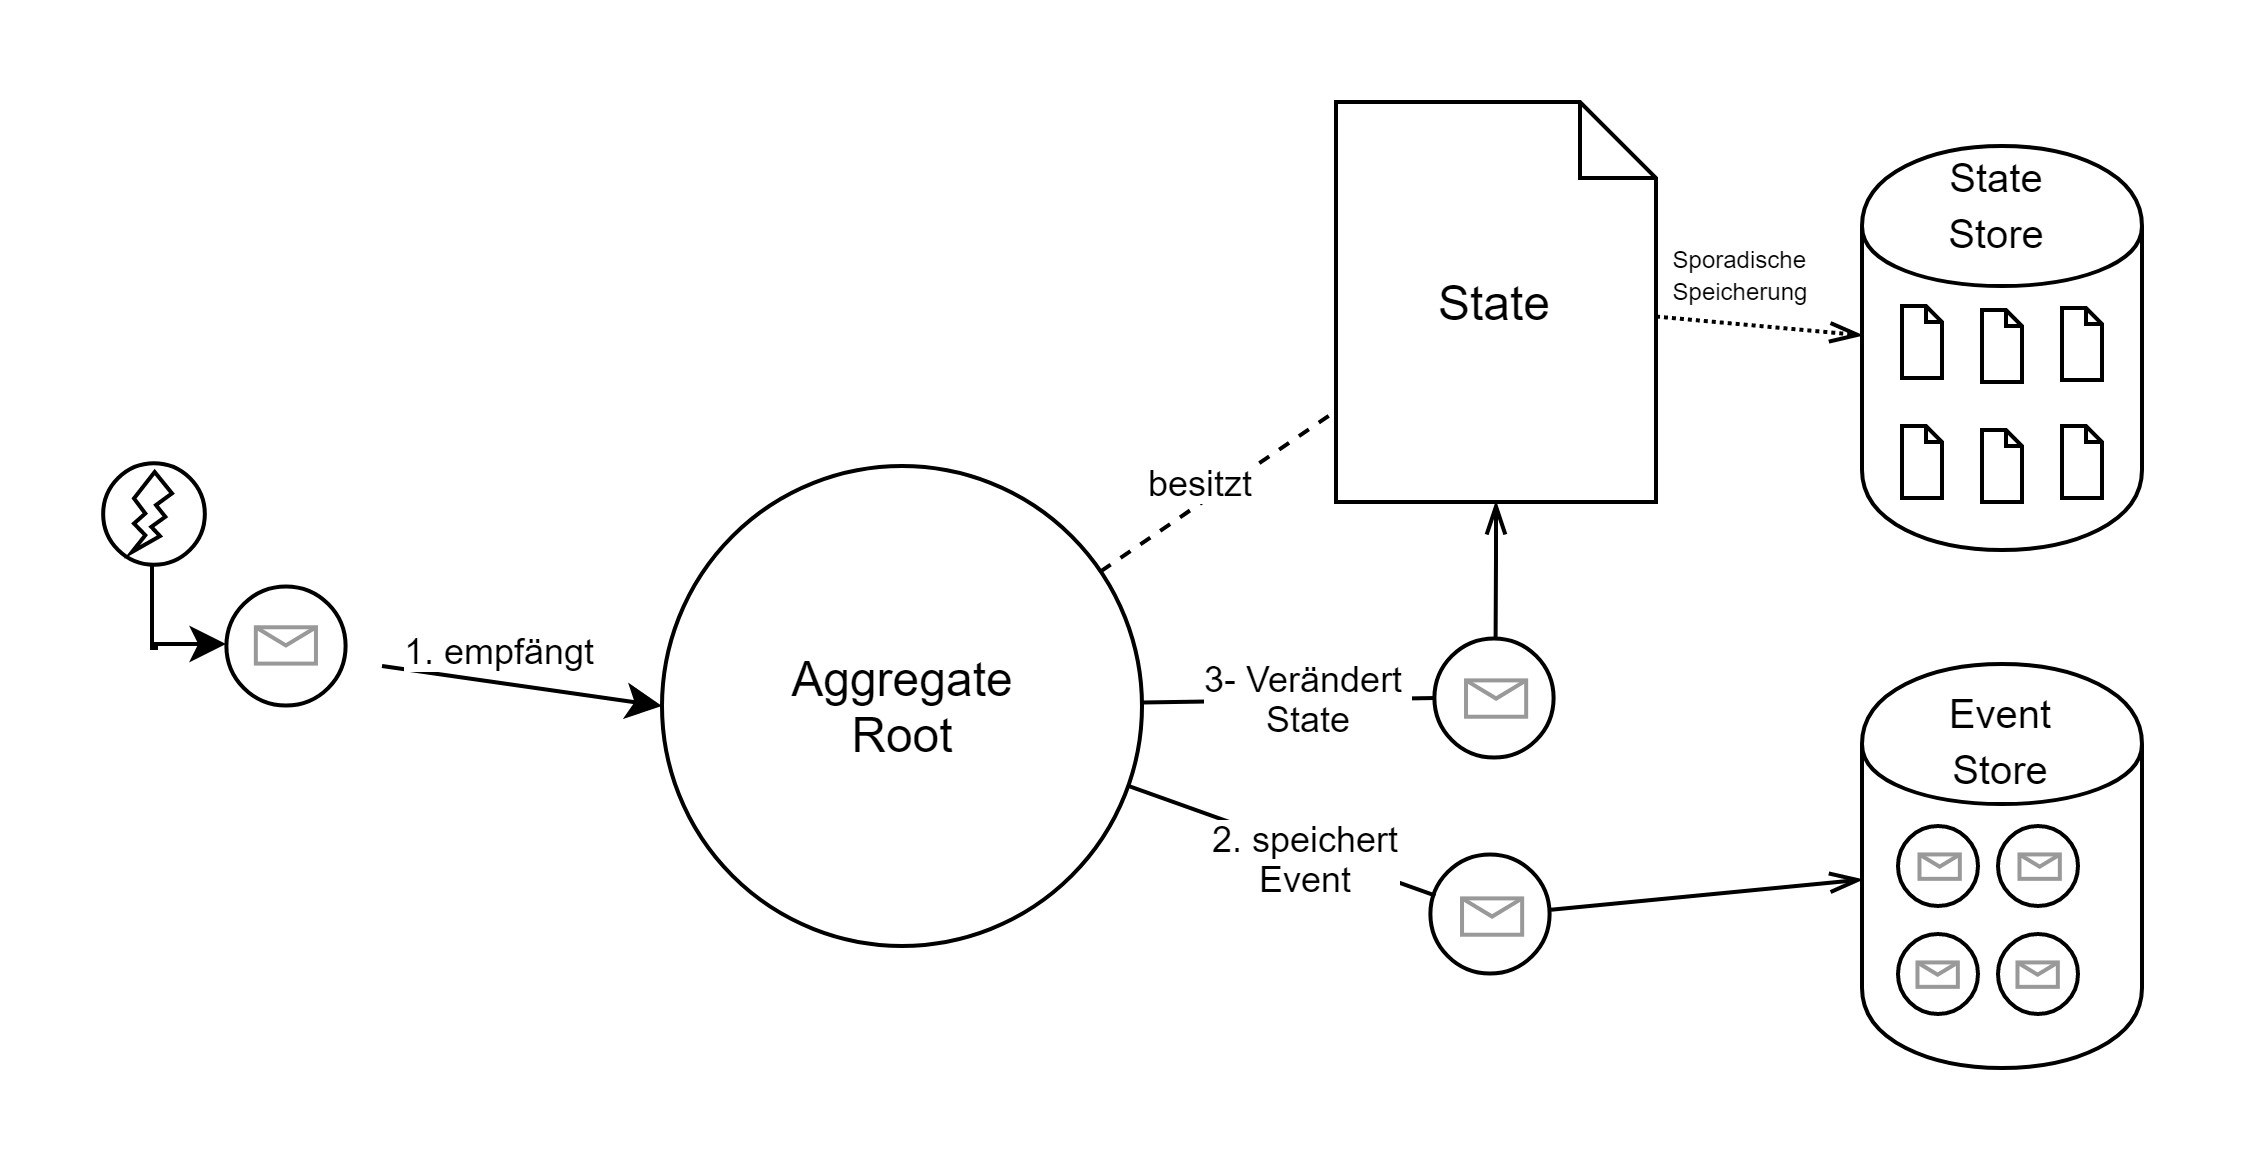
\includegraphics[width=\linewidth]{gfx/implementation/EventSourcingAkka}
  \caption{Ablauf der Speicherung eines Events innerhalb eines \textit{Aggregate Root} Actors mit \textit{Event-Sourcing} und \textit{Snapshots}.}
  \label{fig:implementation:eventSourcingAggregateRoot}
\end{figure} 

\subsection{Snapshot}
\label{subsec:implementation:eventSouring:Snapshot}
Um bei einer Wiedereinspielung der Ereignisse für einen Actor nicht alle bereits aufgetretenen Ereignisse wieder einspielen und dabei für jedes Ereignis die Methode \textit{UpdateState()} aufrufen zu müssen, wird regelmäßig ein Abbild des aktuellen Actorzustands gespeichert. Dies passiert innerhalb der Methode \textit{Emit()}. In der vorliegenden Implementierung wird nach jedem zwanzigsten Event ein \textit{Snapshot} erstellt. Dafür wird die interne Datenrepräsentation eines Actors in eine eigene serialisierbare Klasse, den \textit{Actor State}, abgebildet. Diese Klasse wird auch bei der oben besprochenen Methode \textit{UpdateState()} verändert. Wird nun ein \textit{Snapshot} erstellt, so wird der aktuelle \textit{Actor State} in einer dafür vorgesehenen Datenbank abgespeichert. Zusätzlich zum aktuellen \textit{State} wird die Sequenznummer des letzten Events, welches zu diesem \textit{State} geführt hat, gespeichert. Während der Erstellung des \textit{Snapshots} kann der Actor selbst jedoch weiterhin Nachrichten abarbeiten. Dies beeinträchtigt nicht die Konsistenz der Datenrepräsentation. Durch die Zuordnung von einer Sequenznummer zu einem abgespeicherten \textit{State} werden Events, welche während der Erstellung des \textit{Snapshots} anfallen, nicht mehr zum \textit{Snapshot} dazu gezählt und somit später wieder auf Basis des vorhandenen \textit{Snapshots} eingespielt. \\
Wird nun ein gestoppter Actor, dessen Zustand mittels \textit{Event-Sourcing} persistiert wurde, wieder gestartet, so kommt es zur Wiederherstellung des vorherigen Zustand. Während vergangene Ereignisse eingespielt werden, kann der Actor keine neuen Nachrichten verarbeiten. Diese verbleiben solange in der Mailbox des Actors bis die Einspielung abgeschlossen ist. \\
Die Wiederherstellung eines Actors wird erreicht, in dem zuerst der zuletzt verfügbare \textit{Snapshot} für den Actor in der Datenbank gesucht wird. Anschließend wird der Zustand des entsprechenden \textit{Snapshots} dem Actor als \textit{State} zugeteilt. Nun werden alle Events, welche nach der Erstellung des \textit{Snapshots} angefallen sind, in der zeitlichen Reihenfolge ihres Auftretens wieder in den Actor eingespielt. Nach dem letzten eingespielten Event ist der Zustand des Actors exakt der gleiche wie vor dem Stoppen des Actors. \\
Wie bereits angedeutet, wird nicht von allen Actors innerhalb der \textit{TyrolSky}-Anwendung mittels \textit{Event-Sourcing} der aktuelle Zustand gespeichert. Nur Actors, welche einen für die Konsistenz der Anwendung notwendigen Zustand repräsentieren, wurden mit \textit{Event-Sourcing} persistiert. Dies sind folgende Actors: 
\begin{itemize}
  \item{\textit{OperateFlight}}
  \item{\textit{FlightPassengerList}}
  \item{\textit{ChargingCoordinator}}
  \item{\textit{FlightTicket}}
  \item{\textit{FlightNumber}}
  \item{\textit{DistributedUniqueNamingService}}
\end{itemize}
Die ersten fünf genannten Actors sind Teil der Komponente \textit{Domain Service} und repräsentieren die Domäne der \textit{TyrolSky}. Der verbleibende Actor \textit{DistributedUniqueNamingService} dient zur Implementierung der unterschiedlichen \textit{Query}-Aufbereiter des \textit{Query-Services}, welche bereits in Abschnitt \ref{subsubsub:implementation:queryActorModel:resultPreparator} beschrieben wurden.

\subsection{Version Problematik}
Es muss sichergestellt werden, dass Events bei einer späteren Wiedereinspielung gleich behandelt werden als zu dem Zeitpunk, an welchem das Ereignis tatsächlich aufgetreten ist. Ändert sich die Implementierung für einen bestimmten Event-Typ innerhalb der Methode \textit{UpdateState()}, welche auch vergangene Events verarbeitet, kann es zu Inkonsistenzen der Anwendung kommen. Deshalb muss bei einer Anpassung von dem vorhandenem Code der \textit{UpdateState()} Methode entschieden werden, ob dies Codeänderung auch für ältere Events zulässig ist. Wird durch die Codeanpassung ein anderer Actor State als zuvor berechnet, kann nicht mehr der Originalzustand zum Zeitpunk des Ereignisses herbeigeführt werden. \\
Soll ein neues Verhalten für ein bereits vorhandenes Ereignis benötigt werden, wird ein neuer Event-Typ eingeführt. Durch die Versionierung von Event-Typen können keine Inkonsistenzen durch Codeänderungen in das System gebracht werden. 
